
\chapter*{Sampling results for synthetic rotation profiles.}
\label{apndx:rot_split_apnx}

Here we provide the posteriors following sampling of each set of rotational splittings for the synthetic data .


% \begin{figure*}
%     \centering
%     \begin{subfigure}[b]{\textwidth}
%         \centering
%         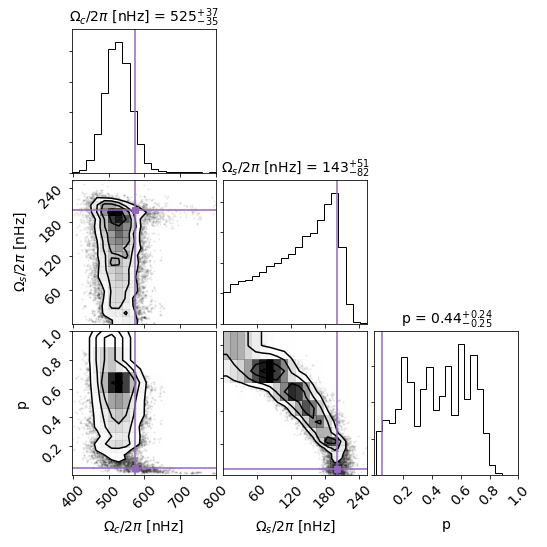
\includegraphics[width=0.475\textwidth]{Figures/subgiant_chapter_figures/10.05_corner.png}
%         \caption[Network2]%
%         {{\small Network 1}}    
%         \label{fig:mean and std of net14}
%     \end{subfigure}
%     \hfill
%     \begin{subfigure}[b]{\textwidth}  
%         \centering 
%         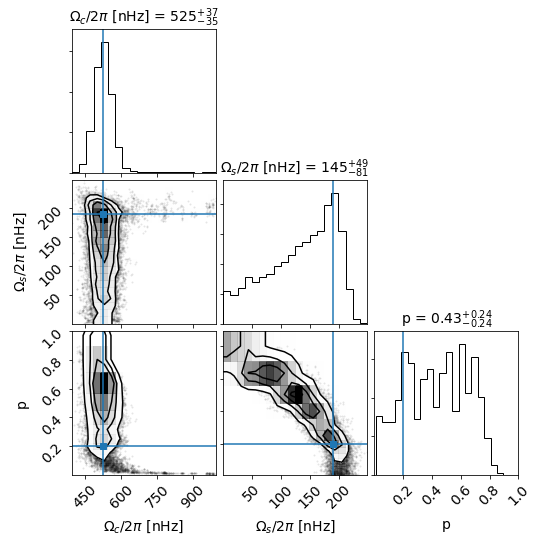
\includegraphics[width=0.475\textwidth]{Figures/subgiant_chapter_figures/10.2_corner.png}
%         \caption[]%
%         {{\small Network 2}}    
%         \label{fig:mean and std of net24}
%     \end{subfigure}
%     \vskip\baselineskip
%     \begin{subfigure}[b]{\textwidth}   
%         \centering 
%         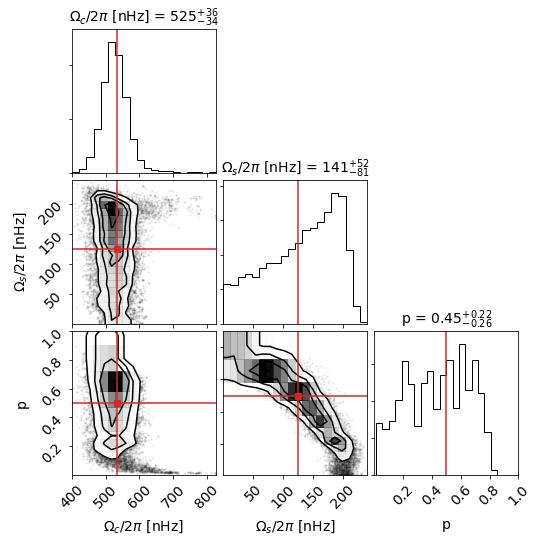
\includegraphics[width=0.475\textwidth]{Figures/subgiant_chapter_figures/10.5_corner.png}
%         \caption[]%
%         {{\small Network 3}}    
%         \label{fig:mean and std of net34}
%     \end{subfigure}
%     \hfill
%     \begin{subfigure}[b]{\textwidth}   
%         \centering 
%         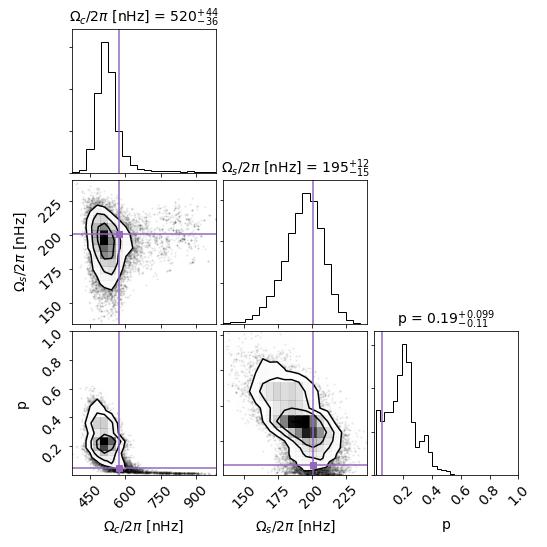
\includegraphics[width=0.475\textwidth]{Figures/subgiant_chapter_figures/20.05_corner.png}
%         \caption[]%
%         {{\small Network 4}}    
%         \label{fig:mean and std of net44}
%     \end{subfigure}
%     \vskip\baselineskip
%         \begin{subfigure}[b]{\textwidth}   
%         \centering 
%         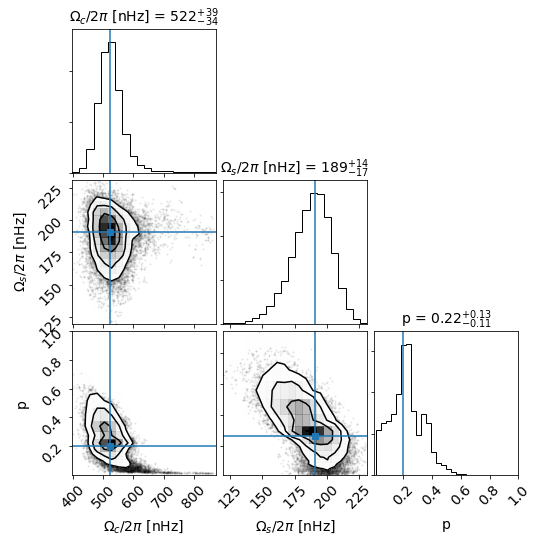
\includegraphics[width=0.475\textwidth]{Figures/subgiant_chapter_figures/20.2_corner.png}
%         \caption[]%
%         {{\small Network 3}}    
%         \label{fig:mean and std of net34}
%     \end{subfigure}
%     \hfill
%     \begin{subfigure}[b]{\textwidth}   
%         \centering 
%         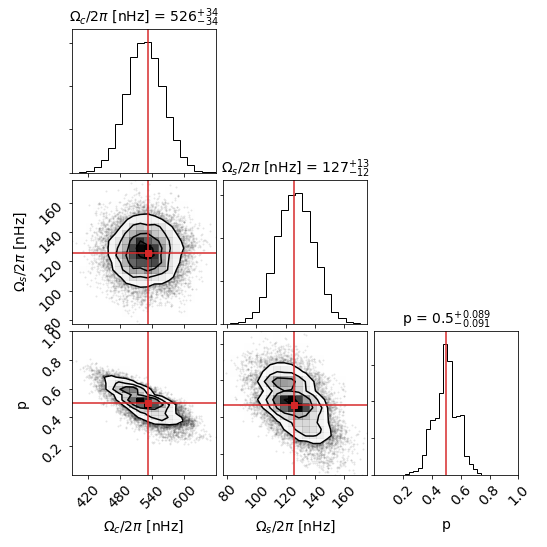
\includegraphics[width=0.475\textwidth]{Figures/subgiant_chapter_figures/20.5_corner.png}
%         \caption[]%
%         {{\small Network 4}}    
%         \label{fig:mean and std of net44}
%     \end{subfigure}
%     \caption[ The average and standard deviation of critical parameters ]
%     {\small The average and standard deviation of critical parameters: Region R4} 
%     \label{fig:mean and std of nets}
% \end{figure*}

\begin{figure}
\centering
    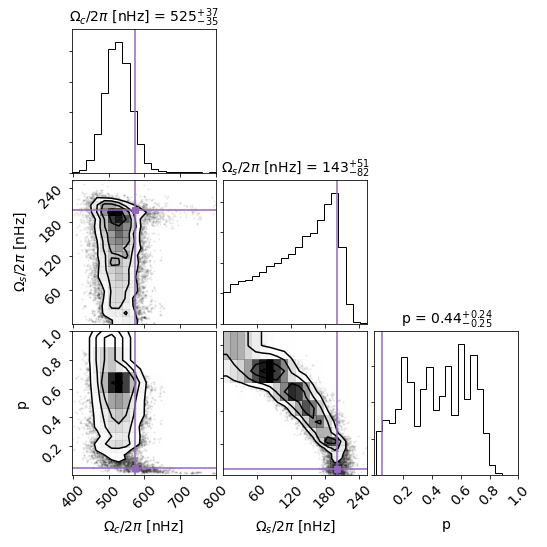
\includegraphics[width=0.5\textwidth]{Figures/subgiant_chapter_figures/10.05_corner.png}
    \caption{
    Posterior distributions using mock data generated with a step function aligned with the H burning shell ($r/R = 0.05$, purple profile in Figure~\ref{fig:5rotprof}). True values are indicated in purple. There is considerable multi-modality and degeneracy present.}
    \label{fig:mock_posterior_005_uniform}
\end{figure}


\begin{figure}
\centering
    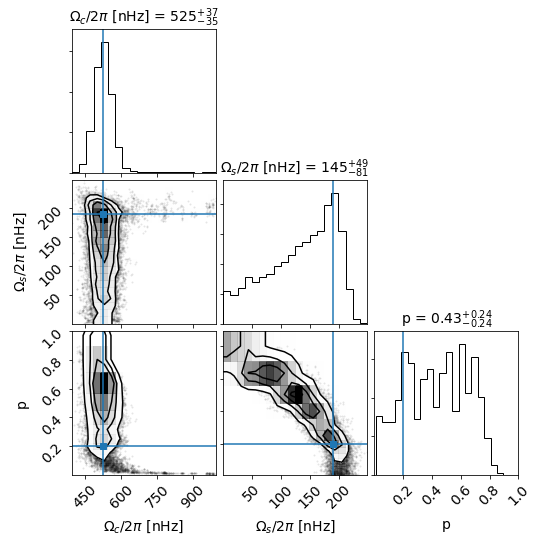
\includegraphics[width=0.5\textwidth]{Figures/subgiant_chapter_figures/10.2_corner.png}
    \caption{Posterior distributions using mock data generated with a step function in the radiative region ($r/R = 0.2$, blue profile in Figure~\ref{fig:5rotprof}) and realistic uncertainties. True values in blue.}
    \label{fig:mock_posterior_020_uniform}
\end{figure}
\begin{figure}
\centering
    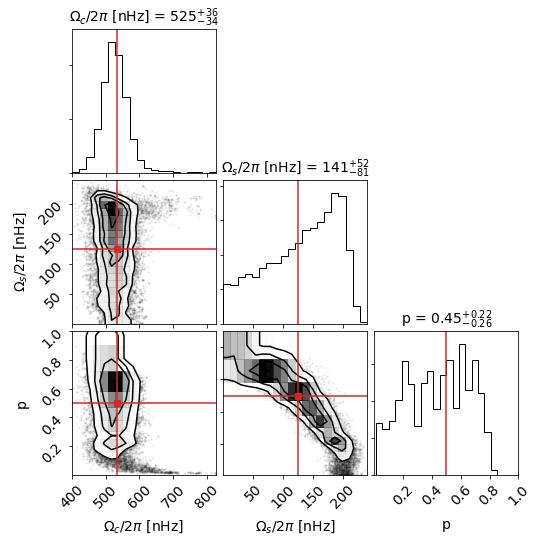
\includegraphics[width=0.5\textwidth]{Figures/subgiant_chapter_figures/10.5_corner.png}
    \caption{Posterior distributions using mock data generated with a step function at the BCZ ($r/R = 0.5$; red profile in Figure~\ref{fig:5rotprof}), and realistic uncertainties. True values in red.}
    \label{fig:mock_posterior_050_uniform}
\end{figure}

\begin{figure}
\centering
    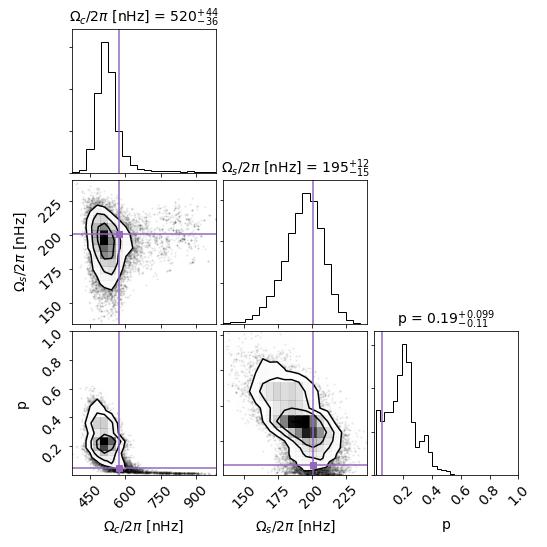
\includegraphics[width=0.5\textwidth]{Figures/subgiant_chapter_figures/20.05_corner.png}
    \caption{Posterior distributions using mock data generated with a step profile at the g-mode cavity ($r/R = 0.05$; purple profile in Figure~\ref{fig:5rotprof}), with realistic uncertainties, and a 10\% prior on surface rotation $\Omega_s$. There is still degeneracy between $p$ and the rotation parameters (e.g., Figure~\ref{fig:mock_posterior_005_uniform}), but the prior has collapsed all other modes.}
    \label{fig:mock_posterior_005_reject}
\end{figure}

\begin{figure}
\centering
    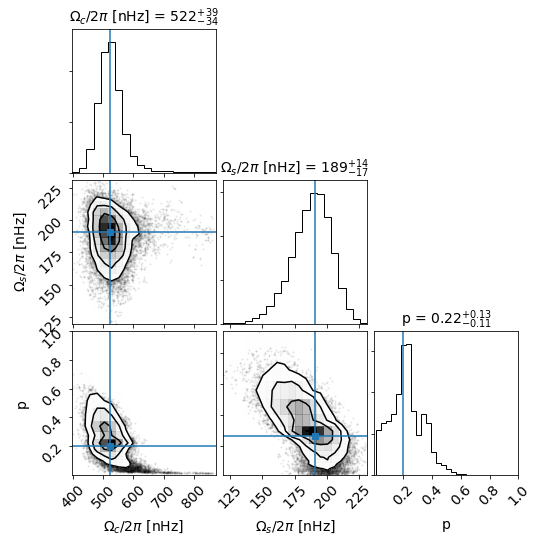
\includegraphics[width=0.5\textwidth]{Figures/subgiant_chapter_figures/20.2_corner.png}
    \caption{Posterior distributions using mock data generated with a step profile in the radiative region ($r/R = 0.20$; blue profile in Figure~\ref{fig:5rotprof}), with realistic uncertainties, and a 10\% prior on surface rotation $\Omega_s$ (compare with Figure~\ref{fig:mock_posterior_020_uniform}).}
    \label{fig:mock_posterior_020_reject}
\end{figure}

\begin{figure}
\centering
    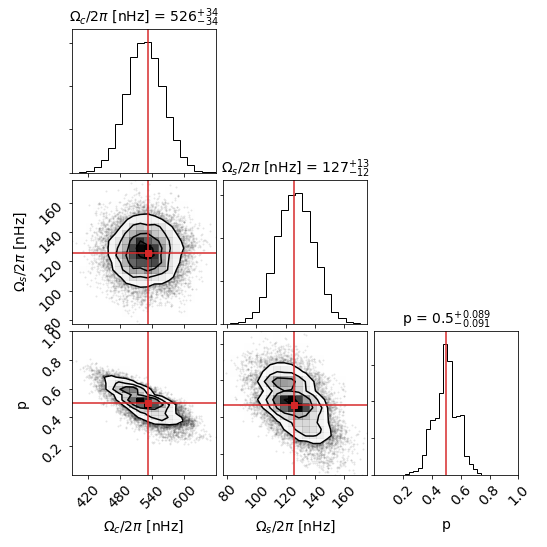
\includegraphics[width=0.5\textwidth]{Figures/subgiant_chapter_figures/20.5_corner.png}
    \caption{Posterior distributions using mock data generated with a step profile at the BCZ ($r/R = 0.50$; red profile in Figure~\ref{fig:5rotprof}), with realistic uncertainties, and a 10\% prior on surface rotation $\Omega_s$ (compare with Figure~\ref{fig:mock_posterior_050_uniform}).}
    \label{fig:mock_posterior_050_reject}
\end{figure}
% Don't change these lines
\bsp	% typesetting comment
\label{lastpage}